\chapter{Dimensions of Experience: Exploring the Heterogeneity of the Wandering Mind}
\chaptermark{Dimensions of Experience}
\label{ch:study1}
\setcounter{equation}{0}

\textit{The following chapter has been adapted from:} Wang, H.-T., Poerio, G. L., Murphy, C. E., Bzdok, D., Jefferies, E., \& Smallwood, J. (2018). Dimensions of Experience: Exploring the Heterogeneity of the Wandering Mind. \textit{Psychological Science}, \textit{29} (1), 56-–71. doi:\url{10.1177/0956797617728727}
\footnote{
J. Smallwood, E. Jefferies, H.-T. Wang, and C. Murphy designed the study. H.-T. Wang, C. Murphy, and G. Poerio collected the data. The connection-strength and sparse canonical-correlation analysis pipeline was constructed by D. Bzdok and H.-T. Wang. Data were analyzed by H.-T. Wang, C. Murphy, and G. Poerio under the supervision of D. Bzdok, J. Smallwood, and E. Jefferies. H.-T. Wang and J. Smallwood drafted the manuscript. G. Poerio and D. Bzdok provided critical revisions. All the authors approved the final version of the manuscript prior to submission.
}\\

% ==========================================================================================================
\newpage

%Abstract
\noindent{}The tendency for the mind to wander to concerns other than the task at hand is a fundamental feature of human cognition, yet the consequences of variations in its experiential content for psychological functioning are not well understood. Here, we adopted multivariate pattern analysis to simultaneously decompose experience-sampling data and neural functional-connectivity data, which revealed dimensions that simultaneously describe individual variation in self-reported experience and default-mode-network connectivity. We identified dimensions corresponding to traits of positive-habitual thoughts and spontaneous task-unrelated thoughts. These dimensions were uniquely related to aspects of cognition, such as executive control and the ability to generate information in a creative fashion, and independently distinguished well-being measures. These data provide the most convincing evidence to date for an ontological view of the mind-wandering state as encompassing a broad range of different experiences and show that this heterogeneity underlies mind wandering's complex relationship to psychological functioning.
% ==========================================================================================================

\section{Introduction}
\label{study1:intro}

Although people's minds frequently wander from events in the here and now, or any task being performed, the functional consequences of this state remain poorly understood \cite{Mittner2016,SeliTiCS2016,SmallwoodFrontiers2013}.
Some studies link mind wandering to unhappiness
\cite{Killingsworth2010};
others suggest it facilitates recovery from negative emotional states
\cite{PoerioFrontiers2016,RubyPlos2013}.
Mind wandering is associated with poorer performance on tasks that place high demands on executive functions
\cite{McVay2009,MrazekJoEP2012},
yet studies of problem solving suggest that mind wandering may promote creativity
\cite{Baird2012,Smeekens2016}.
This wide range of associated functional outcomes is puzzling--—if mind wandering is a homogeneous construct, then it is unclear why it should be associated with such a complex array of often opposing outcomes. To reconcile this contradictory evidence, researchers have suggested that mind wandering may be heterogeneous, encompassing multiple states with differential contents and underlying cognitive architectures \cite{SmallwoodFrontiers2013}. According to this ontological perspective, different functional associations arise from different `types' of experience, which explains the range of functional outcomes observed in the literature.

In the current study, we recruited 165 participants and obtained data on (a) the organization of the brain at rest using functional MRI (fMRI), (b) the content and form of experience recorded across different days, (c) cognitive functions assessed by a comprehensive battery of tasks (including memory, creativity, and executive control), and (d) psychological well-being via questionnaires. Our procedure is presented in Figure \ref{fig:study1:fig1}. These data allowed us to use novel multivariate analysis methods to test the hypothesis that there are different types of mind wandering, with unique neural and experiential patterns accounting for unique variance in the psychological profile of our sample.

\begin{sidewaysfigure}[p]
	\centering
	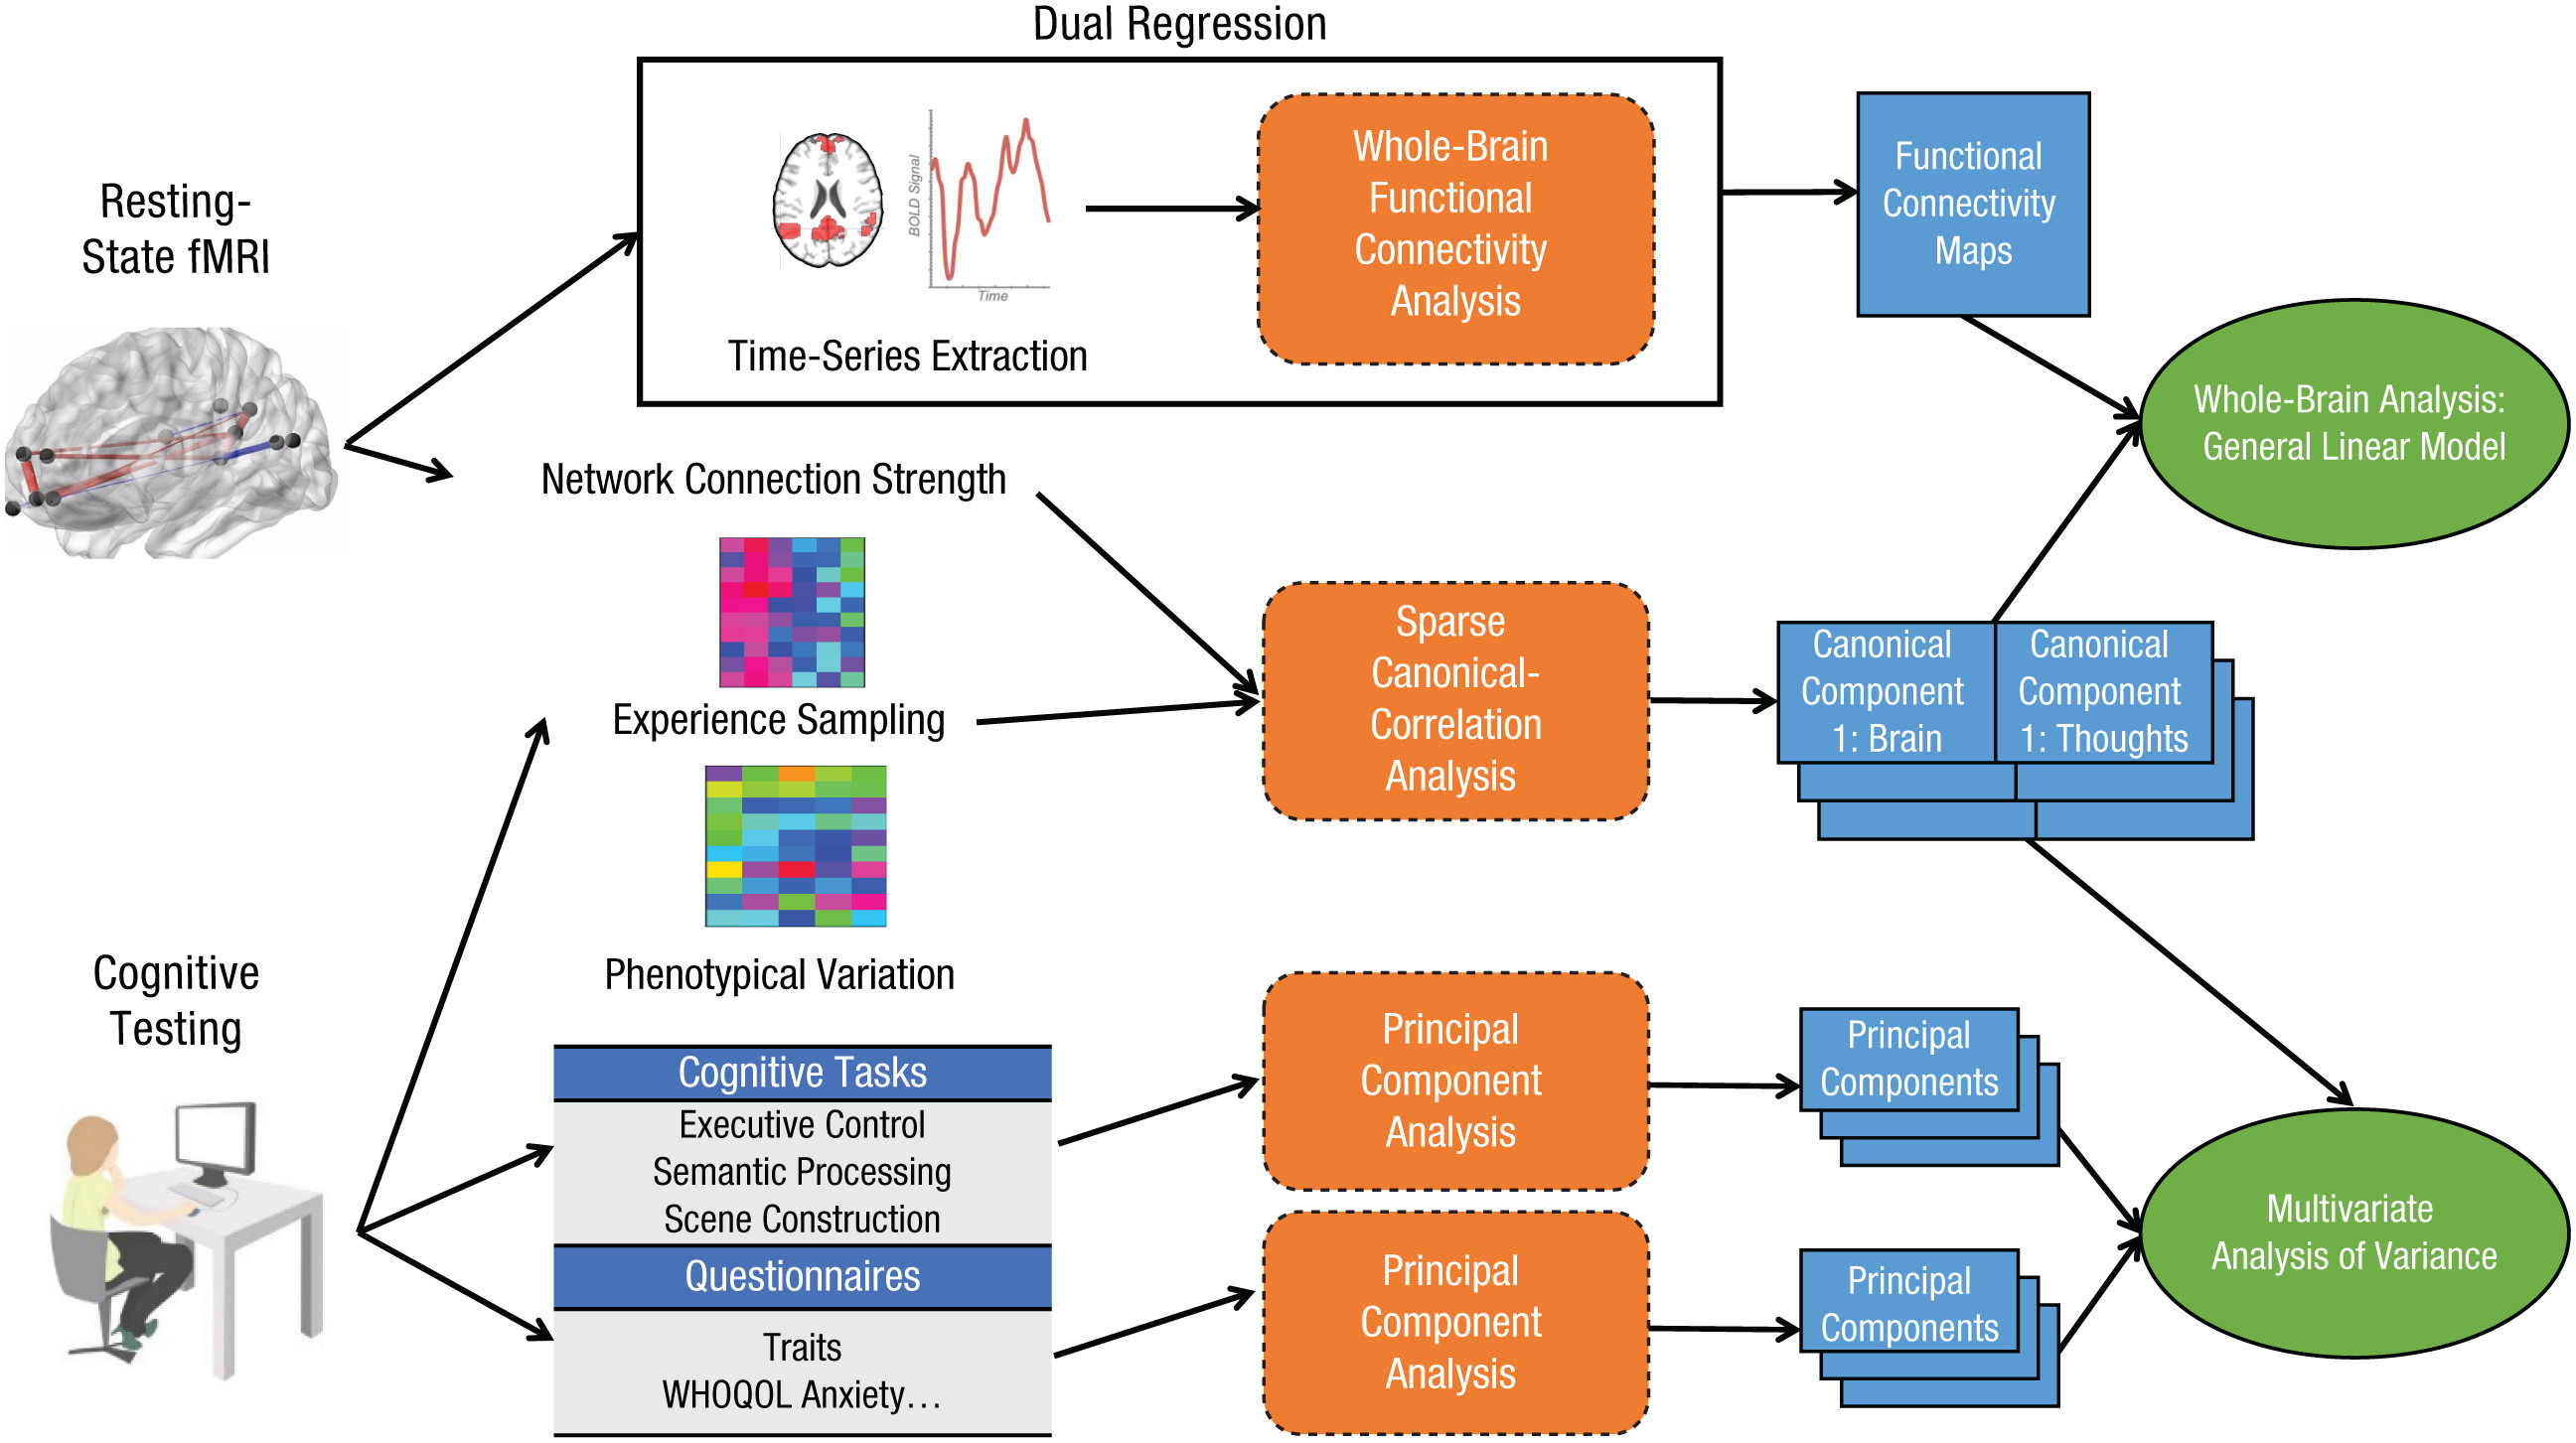
\includegraphics[width=0.8\textwidth]{study1/image/study1fig1.jpeg}
		\caption{Schematic of the procedure and analysis strategy employed in the current study.}
		\caption*{We collected resting-state functional MRI (fMRI) data, cognitive-function measures, and questionnaires on personal traits for each participant. These were submitted to analysis (rectangles with dashed borders), which created latent components or features (rectangles with solid borders) for each subject, and these variables were subsequently passed to the main analysis (ovals). WHOQOL = World Health Organization Quality of Life assessment \cite{WHOQOL2002}.}

	\label{fig:study1:fig1}
\end{sidewaysfigure}

We used functional connection strength to characterize the neural organization of each individual. We selected regions for our analysis on the basis of evidence that task-unrelated thoughts are linked to concurrent increases in activity in medial prefrontal cortex (mPFC), posterior cingulate cortex (pCC), and lateral parietal cortex
\cite<for meta-analyses, see>{Fox2015,Stawarczyk2015}.
—regions that make up the core of the default mode network
\cite<DMN;>{Buckner2008}.
During mind wandering, it is believed that these regions interact with other areas of the cortex, in particular, temporal lobe regions associated with memory representation that are also allied to the DMN. For example, the hippocampus activates early during mind wandering
\cite{Ellamil2016}.
whereas connectivity between lateral and medial aspects of the temporal lobe and the DMN core predicts individual variation in features of mind wandering, such as its episodic content
\cite{Karapanagiotidis2017}.
Contemporary accounts of mind wandering posit that the DMN may be important for automatic aspects of cognition
\cite{Christoff2016}.
Other studies have highlighted links with the lateral prefrontal cortex, which is important for executive control when mind wandering is more deliberate \cite<e.g.,>{Golchert2017}.

We applied multivariate pattern analysis to the neurocognitive and experiential data to identify different types of mind wandering. If the DMN is important for automatic aspects of cognition \cite{Christoff2016}, states linked to high levels of connectivity within this system may have experiential features reflecting more automatic types of cognition. Our a priori decision to focus on the DMN core to derive patterns of experience limited our ability to observe interactions with regions outside of this system, so we used whole-brain functional connectivity to characterize these links for each type of experience. On the basis of prior studies \cite<e.g.,>{Ellamil2016,Golchert2017,Smallwood2016}, we expected this analysis to identify connections with regions in the temporal lobe or the executive system. This pattern would confirm the hypothesised accounts of the DMN as important in integrating neural information \cite{Margulies2016,Smallwood2016}. Having characterised different types of mind wandering in both brain and experience, we used these to test the hypothesis that different categories of experience are related to different functional outcomes. We performed an individual differences analysis to understand whether our characterised types of mind wandering have unique functional associations, including better creativity, worse executive control, and lower levels of well-being. We expected different patterns of experience to capture different psychological profiles explaining the heterogeneous pattern of functional outcomes that have been linked to the mind-wandering state in previous studies
\cite{SmallwoodCC2013}.

% ==========================================================================================================

\section{Method}
\label{study1:method}
\subsection{Participants}
\label{study1:method:a}

One hundred sixty-five healthy participants were recruited from the University of York (99 females, 66 males; age range = 18--31 years, \textit{M} = 20.43, \textit{SD} = 2.63). We preselected a sample size approximately double those used in our prior studies \cite<e.g.>{Smallwood2016}.%(e.g., Smallwood et al., 2016).
A sample size of at least 125 is recommended in order to have 95\% confidence that a correlation of typical size (\textit{r} = .20--.30) is present and greater than 0
\cite{Hemphill2003}.
Participants were right-handed native English speakers with normal or corrected-to-normal vision and no history of psychiatric or neurological illness. Participants underwent MRI scanning, completed an online questionnaire, and then attended three 2-hr behavioural testing sessions to complete a battery of cognitive tasks. The behavioural sessions took place within a week of the scan. Eight participants were excluded from the multivariate pattern analysis because they failed to complete all of the behavioural testing sessions. In total, 157 participants were included in the multivariate pattern analysis and the comparison with cognitive performance. One hundred forty-two participants completed both the behavioural testing sessions and questionnaires and were included in the analysis associated with well-being. Participants were rewarded with either a payment of \pounds 80 or a commensurate amount of course credit. All participants provided written consent prior to the fMRI session and the first behavioural testing session. Approval for the study was obtained from the ethics committee of the University of York Department of Psychology and the University of York Neuroimaging Centre.

\subsection{MRI acquisition}
\label{study1:method:b}
Structural and functional data were acquired using a 3T HDx Excite MRI scanner (GE Healthcare, Little Chalfont, United Kingdom) utilising an eight-channel phased-array head coil tuned to 127.4 MHz at the York Neuroimaging Centre, University of York. Structural MRI acquisition in all participants was based on a T1-weighted 3-D fast-spoiled gradient-echo sequence— repetition time (TR) = 7.8 s,
echo time (TE) = minimum full,
flip angle = \ang{20},
matrix size = 256 $\times$ 256, 176 slices,
voxel size = \SI[product-units=power]{1.13 x 1.13 x 1}{\mm}.
Resting-state activity was recorded from the whole brain using single-shot 2-D gradient-echo-planar imaging—TR = 3 s, TE = minimum full,
flip angle = \ang{90},
matrix size = 64 $\times$ 64, 60 slices,
voxel size = \SI[product-units=power]{3 x 3 x 3}{\mm}, 180 volumes.
Participants viewed a fixation cross for the duration of the 9-min fMRI resting-state scan. A fluid-attenuated inversion-recovery (FLAIR) scan with the same orientation as the functional scans was collected to improve co-registration between subject-specific structural and functional scans.


\subsection{Questionnaires}
\label{study1:method:c}

We administered a battery of questionnaires to comprehensively assess a diverse range of trait-level individual differences that have been previously related to mind wandering. These questionnaires captured the trait-like features of participants’ psychological states, particularly aspects of well-being. The complete details of the questionnaires are presented in Appendix \ref{appendix:study1:subsection1}.

\subsection{Behavioural testing sessions}
\label{study1:method:d}
The trait profiles captured by the questionnaires were complemented by measures of performance on a range of cognitive tasks. Behavioural tasks were selected to measure a broad range of cognitive attributes, including semantic and episodic memory, executive control, fluency, and creativity. These measures were assessed in three sessions. Each session began with a task to index the content and form of mind wandering (0-back/ 1-back task), followed by the other cognitive measures. The order of sessions and the order of tasks was counterbalanced across individuals. Details of the 0-back/ 1-back task are presented in the following paragraph. The complete details of the other cognitive tasks are described in Appendix \ref{appendix:study1:subsection2}.

Using a block design, we assessed the contents of experience during mind wandering in the context of a simple task that manipulated working memory load
\cite<see>[for prior published examples of this task]{Konishi2015,Medea2016}.
This task was performed at the beginning of each laboratory session to minimise participant fatigue. Measuring experience over 3 days provided us with a more comprehensive description of participants’ trait-level mind wandering than would have been possible in a single experimental session.

In both tasks, participants completed target and nontarget trials. In nontarget trials, a pair of shapes appeared on screen; the two shapes were separated by a vertical line. The pairs consisted of a circle and a square, a circle and a triangle, and a square and a triangle, each in two different left/right configurations for a total of six possible pairs. Following an unpredictable sequence of nontarget trials, a target trial was presented in which participants had to make a manual response. The target was a small stimulus presented in either blue or red across conditions, with the colour counterbalanced across participants. In the 0-back condition, the target was flanked by one of two shapes, and participants had to indicate which shape matched the target shape by pressing the appropriate button. In the 1-back condition, the target was flanked by two question marks, and participants had to respond depending on which side the target shape had been on during the prior trial. Responses were made using the left and right arrow keys. Presentation times for fixation crosses ranged from 1.3 to 1.7 s in steps of 0.05 s, and nontarget presentation times varied from 0.8 to 1.2 s in steps of 0.05 s. Target presentation times always ranged from 2.1 to 2.5 s in steps of 0.05 s, and a response from participants did not end the target presentation.

There were eight blocks in one session, and each block consisted of two to four miniblocks. Each block contained either the 0-back or 1-back condition. The change of task was signalled by the presentation of the word “SWITCH,” which remained on screen for 5 s. The order of the tasks was counterbalanced across participants, and the eight blocks lasted around 25 min. In each mini-block, there was one target trial, and the number of nontarget trials preceding the targets varied between one and six. Participants’ performance was measured by their efficiency, which was calculated by dividing their average response time by their accuracy. For ease of interpretation, efficiency scores were reversed, so that higher scores indicated better performance.

In order to sample different features of participants’ ongoing experiences, we used multidimensional experience sampling
\cite<MDES;>{Medea2016,RubyPlos2013,Smallwood2016}.
This technique uses self-report data to assess the contents of experience on a number of dimensions. The first thought probe asked participants to rate their level of task focus (“My thoughts were focused on the task I was performing”) on a sliding scale from 0 (\textit{completely off task}) to 1 (\textit{completely on task}). Participants then answered 12 randomly presented questions regarding the content and form of their experience at the moment just before they answered the first thought probe (on level of task focus). These questions (described in Table \ref{tab:study1:1}) were based on those used in prior studies adopting this approach to measure self-generated thought
\cite{Medea2016,RubyPlos2013,Smallwood2016}.
At the moment of target presentation, there was a 20\% chance of a thought probe being presented instead of a target, with a maximum of one probe per block of the 0-back/1-back task. In each session, an average of 14.07 (\textit{SD} = 3.30, range = 6--25) MDES probes occurred; in the 0-back condition, an average of 7.02 (\textit{SD} = 2.36, range = 2--14) MDES probes occurred; and in the 1-back condition, an average of 7.04 (\textit{SD} = 2.24, range = 1--15) occurred. In total, we sampled 7,006 examples of experience in this study. We calculated the mean scores of each question across the three sessions for each participant. The MDES scores were first transformed into z scores for mean-centring and univariance scaling. The scores described the average momentary experience in each dimension. We used this score in the multivariate analysis later.

\linespacesmall
\begin{table}
\centering
\caption{Experience-Sampling Questions in the 0-Back/1-Back Task.}
\label{tab:study1:1}
\resizebox{\textwidth}{!}{
\begin{tabular}{ l l c c}
\toprule
& & \multicolumn{2}{c}{Response scale} \\ \cmidrule{3-4}
Dimension & \multicolumn{1}{c}{Question} & 0 & 1 \\ \midrule
Focus & My thoughts were focused on the task I was performing.  & \textit{Not at all} & \textit{Completely} \\
Future & My thoughts involved future events. & \textit{Not at all} & \textit{Completely} \\
Past & My thoughts involved past events. & \textit{Not at all} & \textit{Completely} \\
Self & My thoughts involved myself. & \textit{Not at all} & \textit{Completely} \\
Other & My thoughts involved other people. & \textit{Not at all} & \textit{Completely} \\
Emotion & The content of my thoughts was: & \textit{Negative} & \textit{Positive} \\
Images & My thoughts were in the form of images. & \textit{Not at all} & \textit{Completely} \\
Words & My thoughts were in the form of words. & \textit{Not at all} & \textit{Completely} \\
Vividness & My thoughts were vivid as if I was there. & \textit{Not at all} & \textit{Completely} \\
Detail & My thoughts were detailed and specific. & \textit{Not at all} & \textit{Completely} \\
Habit & This thought has recurrent themes similar to those I have had before. & \textit{Not at all} & \textit{Completely} \\
Evolving & My thoughts tended to evolve in a series of steps. & \textit{Not at all} & \textit{Completely} \\
Deliberation & My thoughts were: & \textit{Spontaneous} & \textit{Deliberate} \\ \bottomrule
\end{tabular}
}
\end{table}
\linespacenormal

\subsection{Neuroimaging data preprocessing and analysis}
\label{study1:method:e}

\subsubsection{Resting-state fMRI.}

Functional and structural data were preprocessed and analysed using the Oxford Centre for Functional MRI of the Brain’s (FMRIB’s) Software Library (FSL Version 4.1, \url{http://www.fmrib.ox.ac.uk/fsl}).
Individual FLAIR and T1-weighted structural brain images were extracted using FSL’s Brain Extraction Tool (BET). Structural images were linearly registered to the MNI152 template using FMRIB’s Linear Image Registration Tool (FLIRT). The resting-state functional data were preprocessed and analysed using FSL's FMRI Expert Analysis Tool (FEAT). The individual-subject analysis involved motion correction using FSL’s MCFLIRT, slice-timing correction using Fourierspace time-series phase shifting, high-pass temporal filtering (Gaussian-weighted least-squares straight-line fitting, \(\sigma\)= 200 s), and Gaussian low-pass temporal filtering (\(\sigma\) = 2.8 s). In addition, we regressed out six motion parameters (as estimated by MCFLIRT) and regressing out cerebrospinal fluid and white-matter signal (top five components in the principal component analysis, PCA; CompCor method). No spatial smoothing and no global signal regression were applied.

\subsubsection{Network-strength analysis.}

To describe the functional architecture of the DMN, we transformed the resting-state blood-oxygen-level-dependent time series into connection strength values of the selected regions for each participant. The regions of interest (ROIs) were obtained from connectivity-based functional parcellation studies of the DMN by Bzdok and colleagues
\cite{BzdokNI2013,Bzdok2015,Bzdok2016,Eickhoff2016,Eickhoff2016}.
There were 16 selected target network nodes, including subregions located in the bilateral temporoparietal junction (TPJ), ventromedial prefrontal cortex (vmPFC), dorsomedial prefrontal cortex (dmPFC), and posteromedial cortex
(PMC; see Fig.\ref{fig:study1:fig2}a).
The ROI masks and the related functional-connectivity network produced with Neurosynth core tools
(\url{http://github.com/neurosynth/neuro_synth})
can be found on NeuroVault
(\url{http://neurovault.org/collections/2275/}). First, we extracted and then averaged the time series of all voxels within the 6-mm sphere masks of the given regions. Second, we created \(16\times16\) symmetrical correlation matrices representing the network of the regions that was computed for all the individual subjects. The off-diagonal of each correlation matrix contained 120 unique region-region connection strengths. This approach provided a measure of connection strength of the region-region coupling of the DMN for each participant.

\begin{sidewaysfigure}[p]
	\centering
	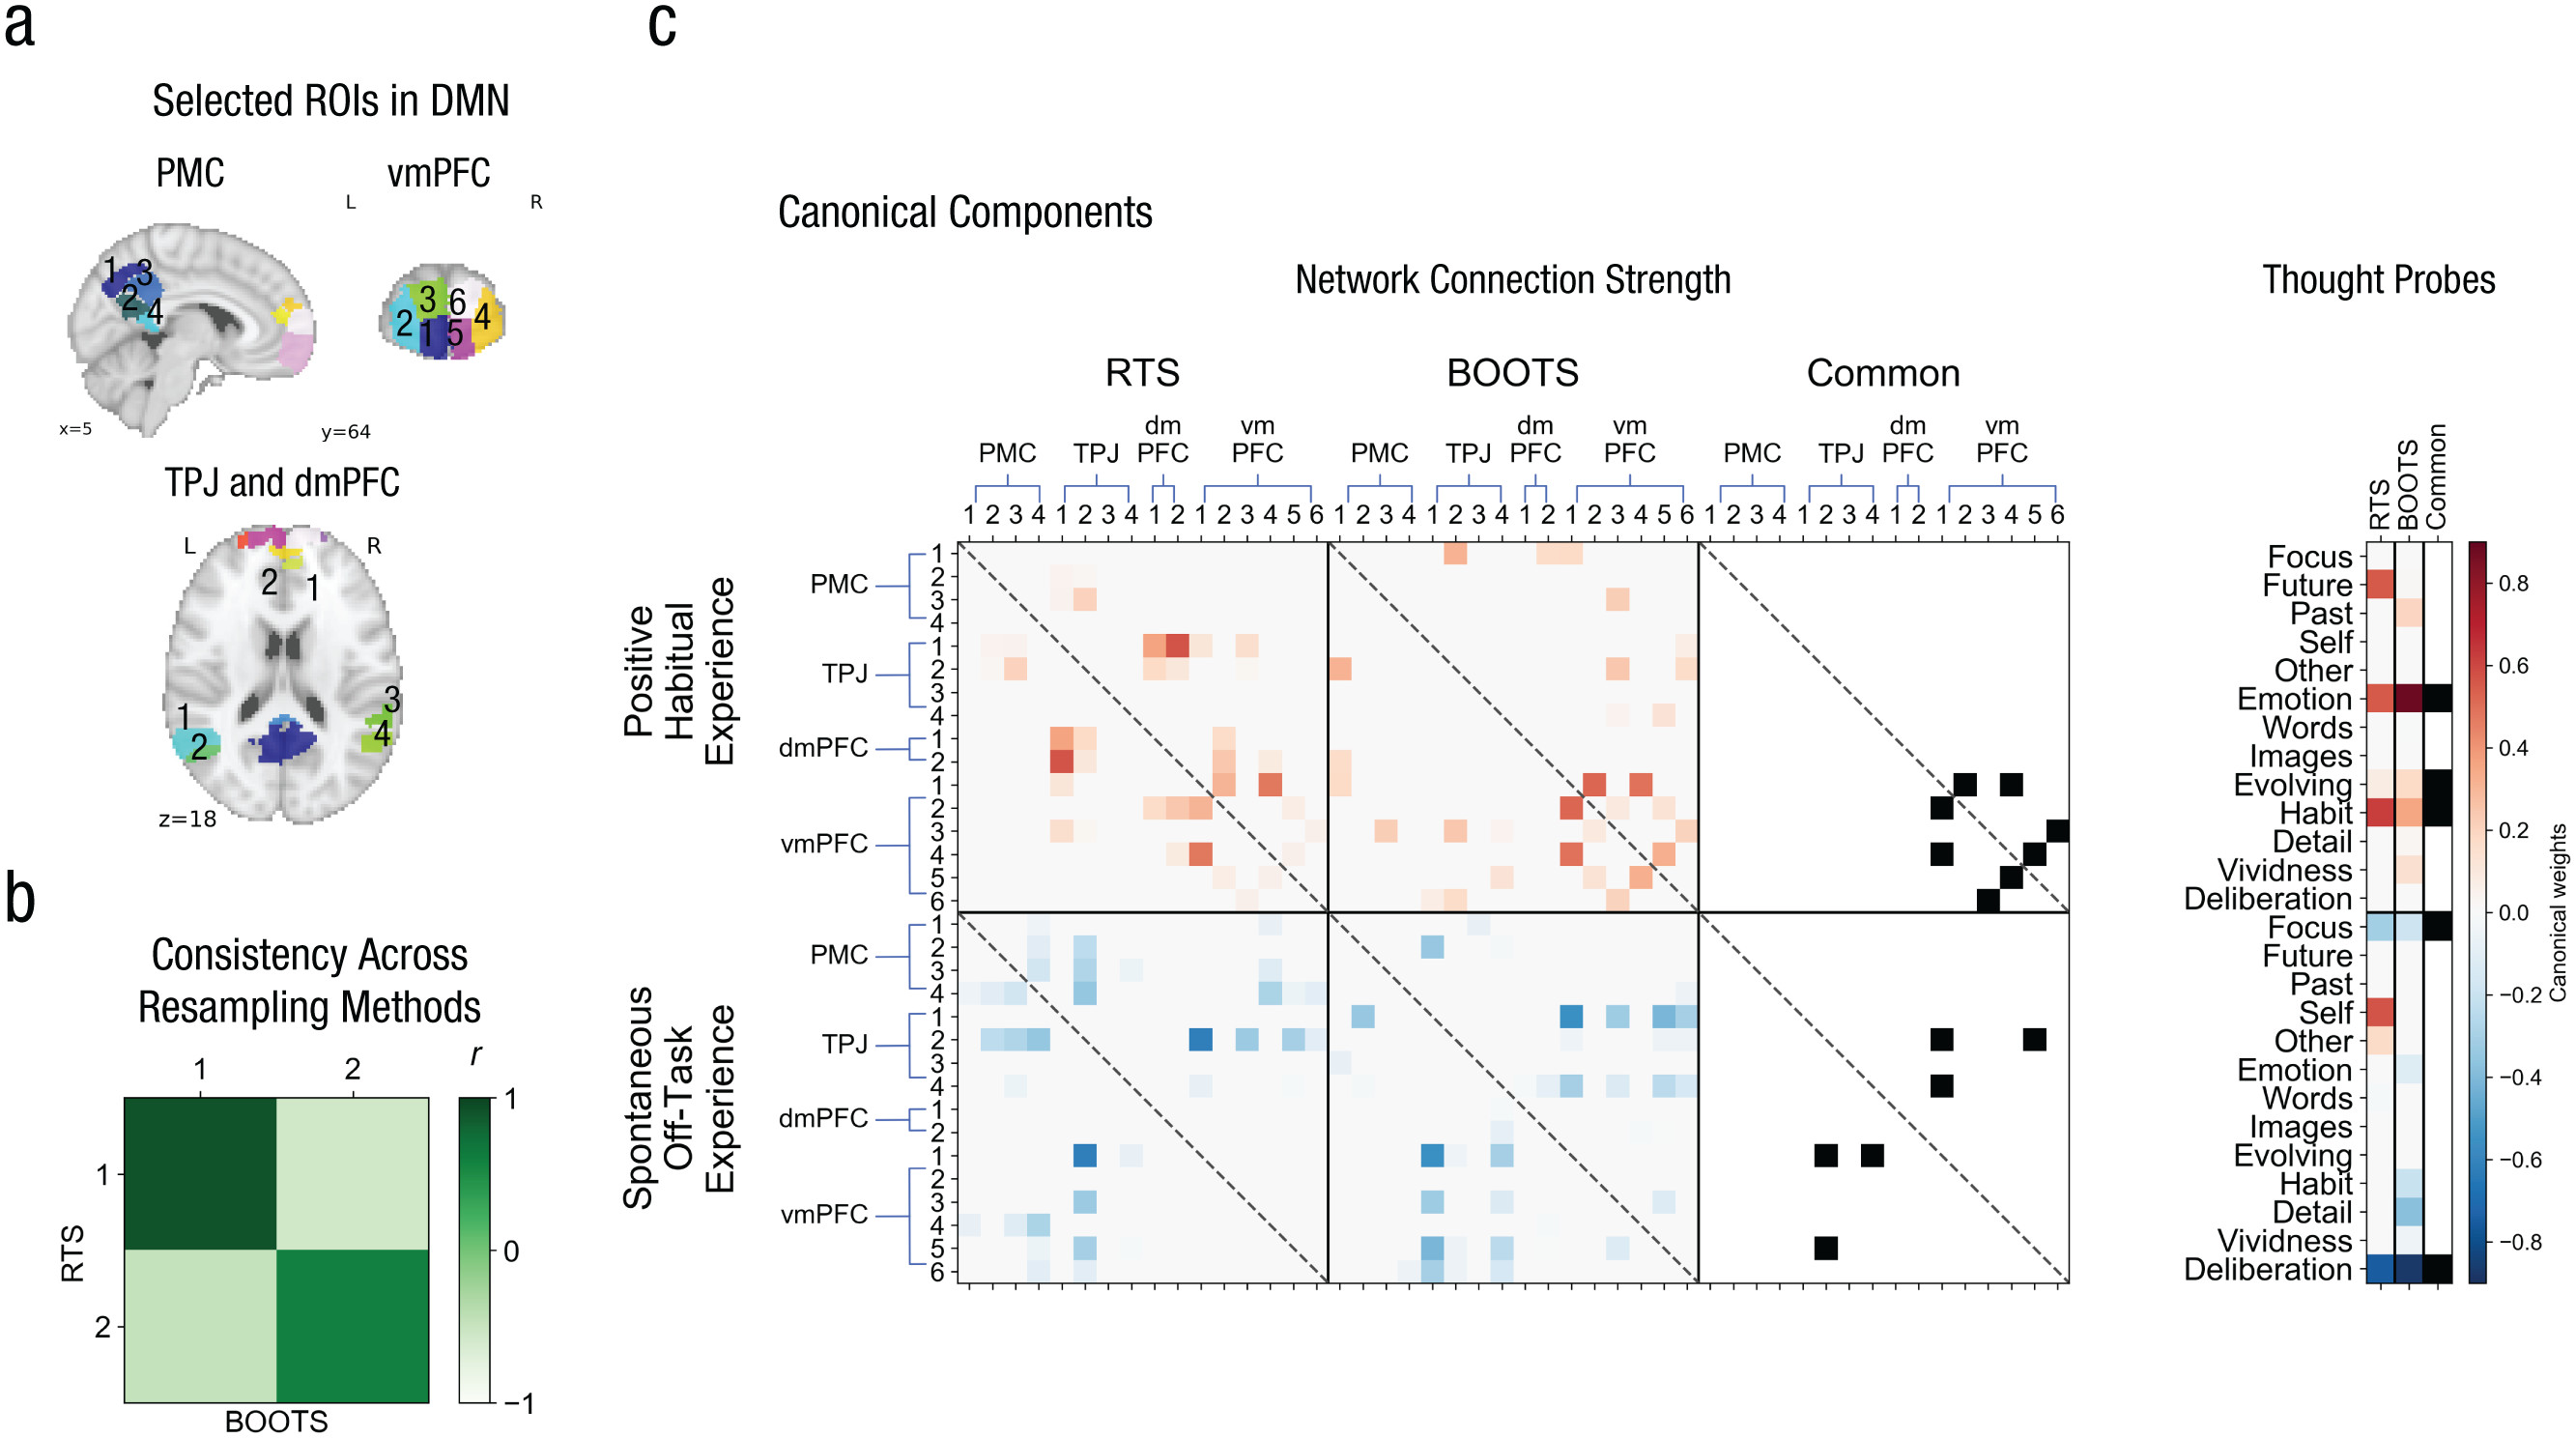
\includegraphics[width=0.8\textwidth]{study1/image/study1fig2.jpeg}
	\caption{Results of the sparse canonical-correlation analysis.}
	\caption*{\scriptsize{The regions of interest (ROIs) of the default mode network (DMN) from which the network connection strength was calculated are shown in (a). The correlation between the two canonical components (positive-habitual experience, 1, and spontaneous off-task experience, 2) and the two analyses is shown in (b). The analyses were restricted temporal sampling (RTS), which describes the canonical components produced when the data from 1 day of each participant were randomly removed from the decomposition, and bootstrapping (BOOTS), which describes the solution produced using bootstrapping. Panel (c) shows the results of the sparse canonical-correlation analysis (SCCA) conducted on the network-connection-strength values of key nodes of the DMN at rest and self-reports of experience during a laboratory task. Results are shown separately for the two components of experience for each analysis. Also shown are the common findings between the two analyses. The numbers indicate the subregions of each ROI, as indicated in (a). For the questions associated with each self-report dimension, see Table 1. PMC = posteromedial cortex, vmPFC = ventromedial prefrontal cortex, TPJ = temporoparietal junction, dmPFC = dorsomedial prefrontal cortex.}}

	\label{fig:study1:fig2}
\end{sidewaysfigure}

\subsubsection{Multivariate pattern analysis.}

We performed a sparse canonical-correlation analysis (SCCA) on the connection strength data and MDES scores to yield different dimensions that simultaneously described neural organisation and experience. Canonical correlation analysis (CCA) is an advanced multivariate technique that identifies distinct components between two variables spaces \cite{Hardoon2004}--in our case, brain-region connection-strength values and experiential reports obtained through MDES. This modelling approach allows linear combinations of the two variable vectors with correlations among variables to be determined and, unlike in PCA and independent component analysis, produces dimensions in which the biological data are simultaneously constrained by psychological measures (and vice versa). To enhance the interpretability of the decomposition solutions, we used a variant of CCA penalised by L\textsubscript{1} regularisation, SCCA \cite<see>{Hastie2015}. This was achieved by setting a maximum number of brain or behaviour variables to exactly zero, which resulted in a regularised version of the singular value decomposition. A reliable and robust implementation of the SCCA method was retrieved as an R package from CRAN (penalized multivariate analysis, or PMA). In the current analysis, the L\textsubscript{1} penalty was set to 0.3 on resting-state functional connectivity and to 0.5 for the MDES results. Other parameters were set to the default. In this way, our analysis performed low-rank (i.e., described an overall network pattern by a parsimonious set of connectivity causes), conjoint (i.e., respected variance in brain and behaviour at once), and sparse (i.e., automatically found unimportant variables) decomposition of experiential and neural data.

\subsubsection{Stability analyses.}

We performed two analyses to assess the stability of the solutions produced by SCCA. First, for each participant, we excluded the MDES data of 1 random day and then recalculated the average scores for these questions. We repeated the decomposition on this new set of MDES data and the network connection strength. This corroborative quantitative assessment provided insight into the robustness of the obtained findings by a permutation analysis that left 1 day out at a time. In particular, this procedure addressed whether either the first day (when participants may be learning how to respond to the experience-sampling method) or the last day (when participants may have lower levels of motivation) might unduly bias the decomposition solutions. We reasoned that if the average momentary MDES responses are stable across three sessions, then they should yield similar latent components. Second, we acquired bootstrap samples as a permutation analysis to estimate the variance and generalisability of the sample to the population. The bootstrap resamples, each reflecting an alternative data sample that we could have obtained from the same distribution, was created by random sampling with replacement. The identical SCCA computation was then reiterated individually on each of the 1,000 perturbed versions of the actual data sample. This approach enables quantitative assessment of the quality of the original SCCA estimates by inferring confidence intervals (see Fig.\ref{fig:3S1} in the Appendix \ref{appendix:study1:subsection3} for the distributions). We selected latent components that were consistent across the decomposition of the original sample, a leave-1-day-out sample, and a bootstrap sample, as those are the stable components that were less biased by the session effect and closer to our best estimation of population. We formalised the similarity of these two types of resampling by conducting a formal conjunction of the solutions generated through these different methods of resampling. To quantify the similarity between the components, we performed a conjunction that highlights the common elements of each solution. The feature conjunctions were calculated as follows:

\begin{equation}
  \text{conjunction}=
  \begin{cases}
    1, & \text{when}
    \sqrt{
    \text{canonical weight\textsubscript{LODO}}
    \times
    \text{canonical weight\textsubscript{BOOTS}}
    } < 0.1\\
    0, & \text{otherwise}.
  \end{cases}
\end{equation}

where LODO refers to leave 1 day out and BOOTS refers to bootstrapping. In addition, because bootstrapping produces a population estimation of our sample, we used the latent component weights produced by this method to compute component scores. This set of scores was used in all subsequent analyses. The source code for this analysis is available at \url{https://github.com/ htwangtw/DimensionsOfExperience}.

\subsubsection{Whole-brain analysis.}

A limitation in our analysis is that we focused on the DMN to describe patterns of thought. To overcome this limitation, we generalised the types of experience provided by the SCCA by assessing their associations with areas outside of the DMN using a process conceptually similar to dual regression \cite{DualRegression2009}. To perform these analyses, we preprocessed and analysed the resting-state functional data using FEAT. For the individual-subject preprocessing procedure, see the Resting-State fMRI section.

Following these preprocessing steps, we used a mask produced by the average of the DMN ROIs to determine the time series that described this neural system. This time series was used in a whole-brain functionality analysis for each participant. This allowed us to produce a subject-specific spatial map based on the selected ROIs, and these maps were used as dependent measures in our group-level analysis. To test whether the functional connectivity of the DMN ROIs was associated with the canonical components, we conducted a group-level analysis using FMRIB’s Local Analysis of Mixed Effects Stage 1 (FLAME 1). To control for spurious correlations that might emerge from movement, we included the two canonical components on thought reports only, group mean and Jenkinson’s mean framewise displacement \cite<FD>{Jenkinson2002}, as explanatory variables in the full model. The Jenkinson’s mean FD was calculated by the motion power statistic function in Configurable Pipeline for the Analysis of Connectomes
(C-PAC; \url{https://fcp-indi .github.io/}).
A 50\% probabilistic gray-matter mask was applied to the results maps, and the results were thresholded at the whole-brain level using cluster-based Gaussian random-field theory, with a cluster-forming threshold (\(\mathit{Z}\)) of 2.6 and a familywise-error-corrected cluster significance level (\(\mathit{p}\)) of .05. Unthresholded maps were uploaded onto Neurovault
(\url{http://neurovault.org/images/43189/}).

\subsubsection{PCA.}
To summarise the questionnaire and task data, we performed an initial data-reduction step using PCA in SPSS (Version 24). This analysis was performed separately for the questionnaires and task measures. One hundred forty-five participants’ data were included in the analysis of the questionnaire items, and 157 participants’ data were included in the analysis of the behavioural tasks. The behavioural-task measures were converted into \(\mathit{z}\) scores to avoid data distortions derived from the difference in score means. Missing data were imputed by mean scores in both analyses. The Kaiser-Meyer-Olkin (KMO) measure and Bartlett’s test of sphericity were used to measure the sampling adequacy of the model. Components were selected on the basis of the elbow in a scree plot (see Fig.\ref{fig:3S2} in Appendix \ref{appendix:study1:subsection3}), and varimax rotation was used to maximise the distinctiveness of each solution.

In the PCA of the phenotypical variation measured by behavioural tasks, Bartlett’s test of sphericity was significant,
\(\chi^{2}(210) = 775.01\),
\(\mathit{p} < .001\),
which indicates that it is appropriate to apply PCA to these data. The KMO measure of sampling adequacy indicated that the current sample was acceptable for PCA (KMO = 0.79). The PCA of task performance revealed three principal components with a clear elbow after the third component observed in the scree plot. The three orthogonal components accounted for 40.7\% of the total variance; the component loading patterns are shown in Figure \ref{fig:study1:fig3}a. The three components, which accounted for 24.9\%, 8.3\%, and 7.5\% of the variance, respectively, can be interpreted as the three aspects of cognitive functioning: (a) semantic memory, (b) executive control, and (c) the generation of information (including letter or category fluency and the generation of creative solutions).

In the PCA of the questionnaire data, Bartlett’s test of sphericity was significant,
\(\chi^{2}(105) = 919.78\),
\(\mathit{p} < .001\),
which indicates that PCA is an appropriate model for the data. The KMO measure of sampling adequacy indicated that there were strong relationships among the variables (KMO = 0.82). The application of PCA to the questionnaire data revealed four components with a clear elbow after the fourth component observed in the scree plot in Fig. S2. The four orthogonal components accounted for 65\% of the total variance (produced component loading patterns are shown in Figure \ref{fig:study1:fig3}b). The four components accounted for 35\%, 14\%, 9\%, and 7\% of the variance, respectively. The first component, affective disturbance, was anchored at one end by high levels of depression and rumination and at the other by high levels of well-being. The second component was associated with high scores on four of the five autism subscales, excluding the attention-to-detail subscale. The third component loaded on components of both attention-deficit/hyperactivity disorder (ADHD) and dyslexia. The fourth component loaded on trait anxiety and high levels of attention to detail, as measured by the Autism Spectrum Quotient \cite{Baron-Cohen2001}. We analysed these data using a multivariate analysis of variance (MANOVA) in which the dependent variables were the PCA loadings produced by the decomposition of the questionnaires, and the independent variables were the canonical component loadings.
\begin{figure}[p]
	\centering
	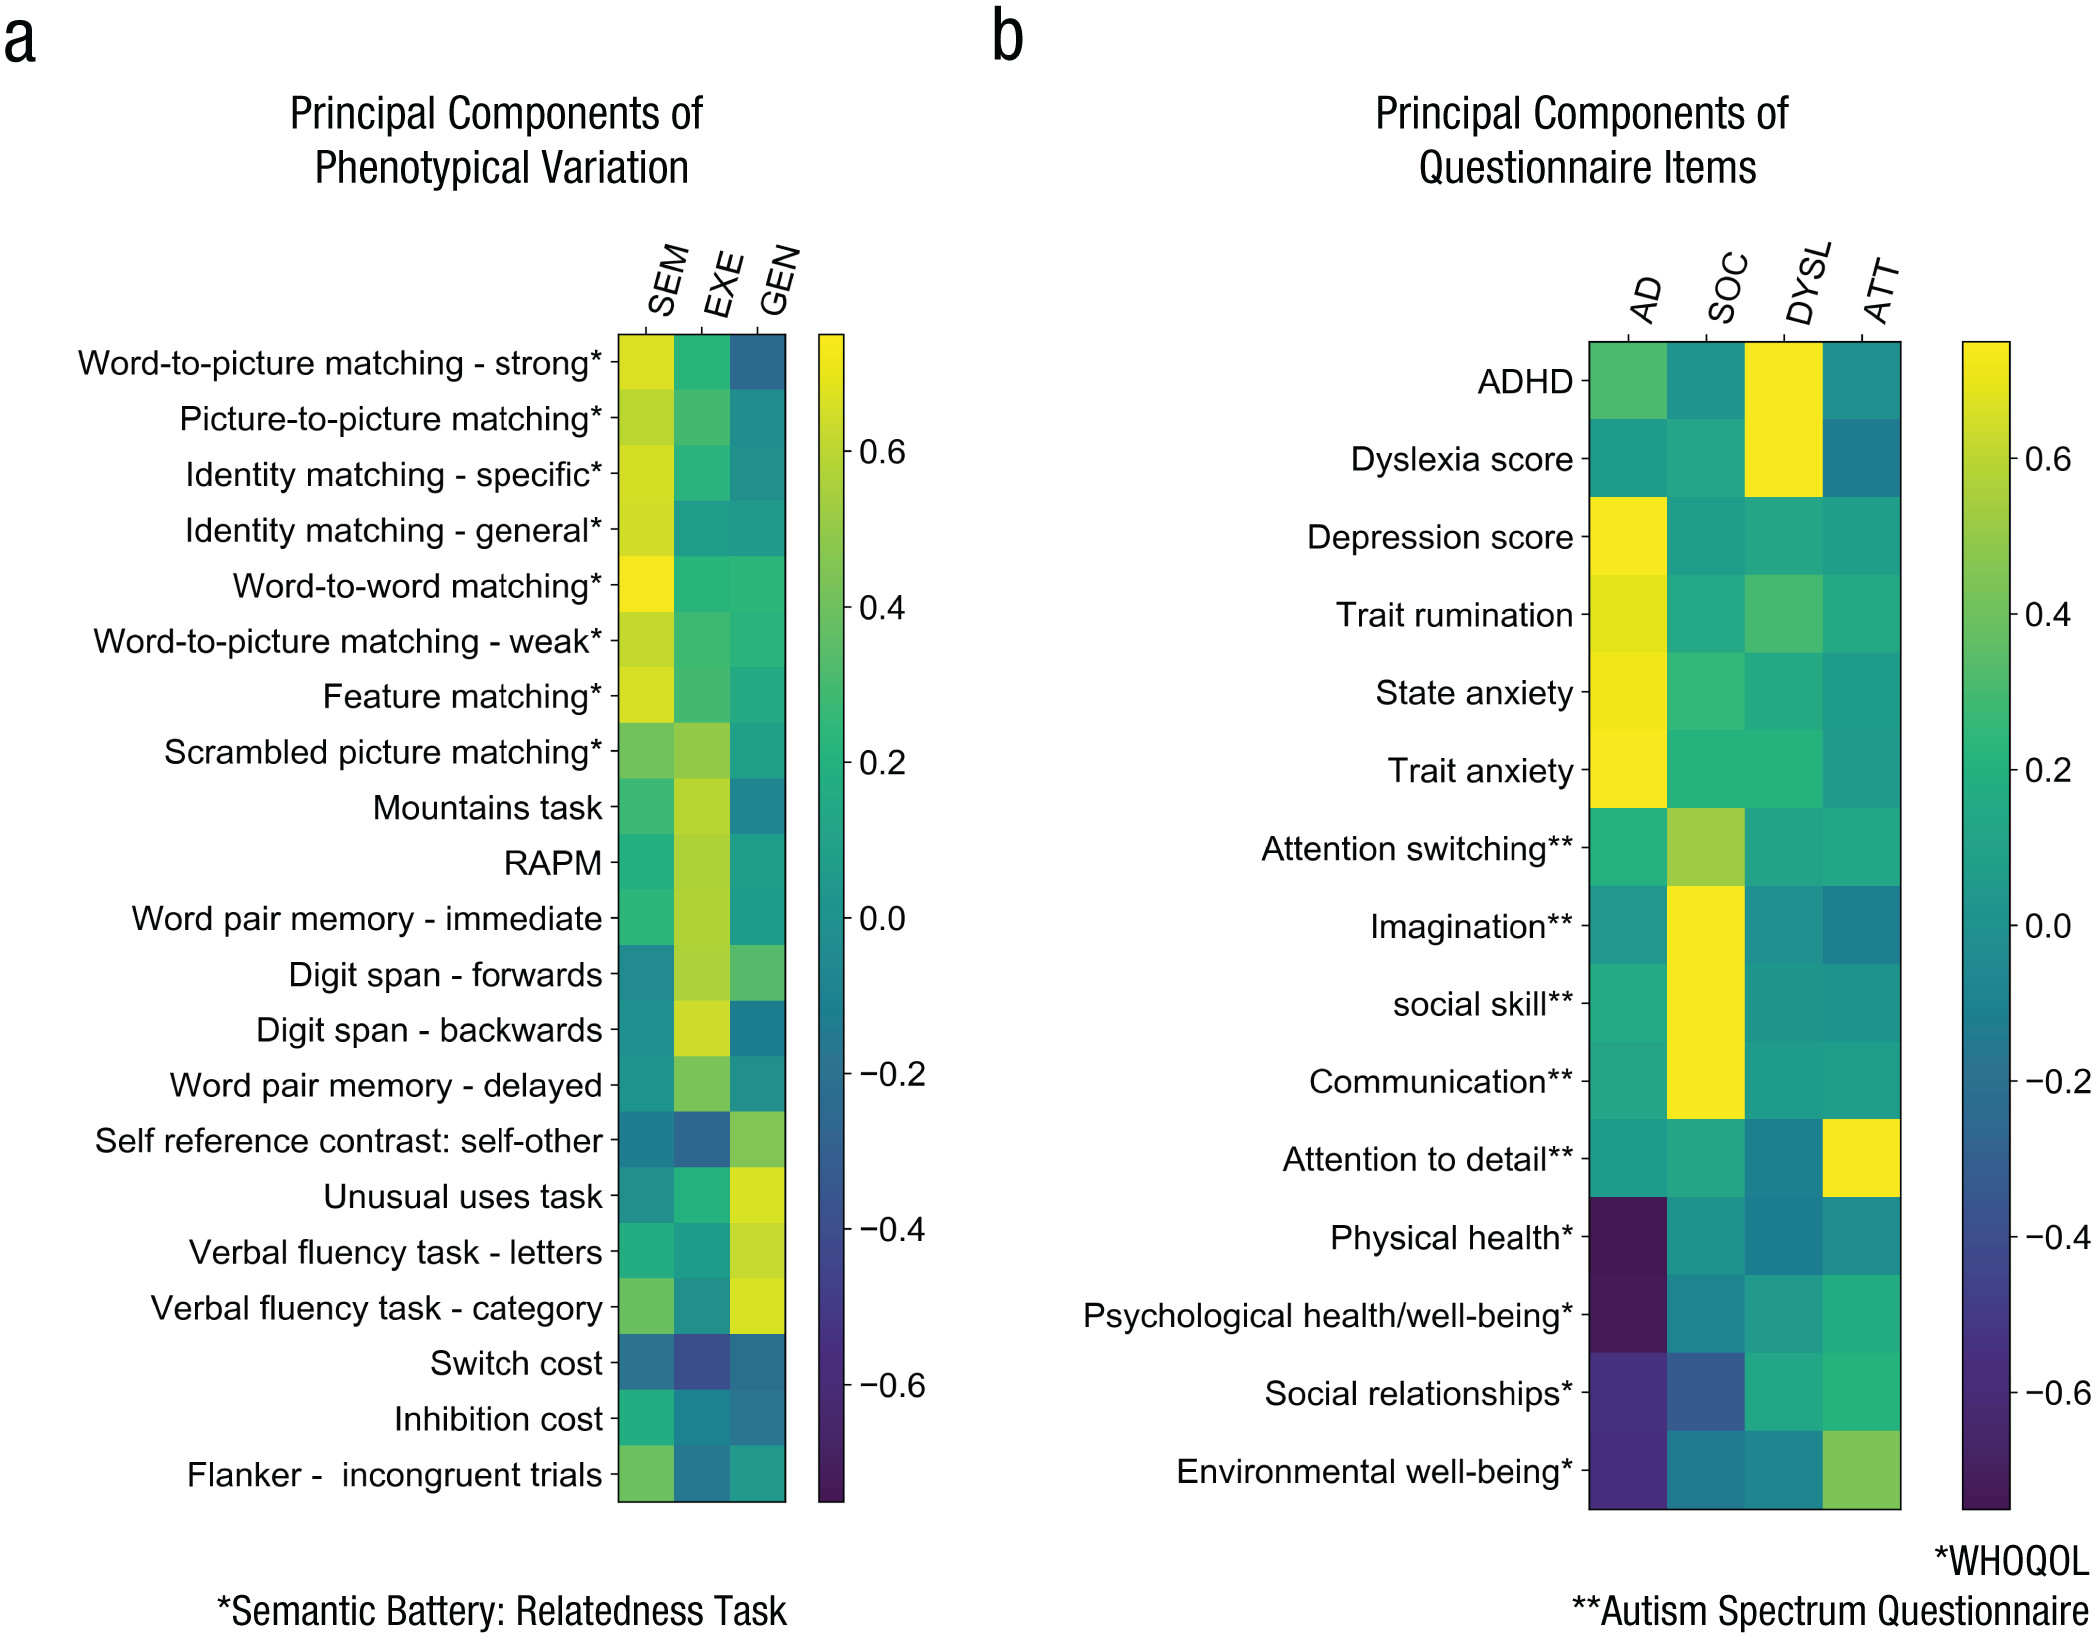
\includegraphics[width=0.8\textwidth]{study1/image/study1fig3.jpeg}
	\caption{Results from principal component analyses of (a) behavioural tasks and (b) questionnaires.}
	\caption*{In the analysis of behavioural tasks, the components were semantic memory (SEM), executive control (EXE), and the generation of information (GEN). In the analysis of questionnaire data, the components were affective disturbance (AD), social interaction (SOC), dyslexia (DYSL), and attention to detail (ATT). The heat map indicates the loadings of each measure. In (a), an asterisk indicates that measures were relatedness tasks from a semantic battery. In (b), a single asterisk indicates measures drawn from the World Health Organization Quality of Life assessment \cite{WHOQOL2002}, and two asterisks indicate measures drawn from the Autism Spectrum Quotient \cite{Baron-Cohen2001}. ADHD = attention-deficit/hyperactivity disorder; RAPM = Raven’s Advanced Progressive Matrices \cite{Raven1998}. For the scree plots describing the eigenvalues for each dimension, refer to Fig.\ref{fig:3S2} in Appendix \ref{appendix:study1:subsection3}.}
	\label{fig:study1:fig3}
\end{figure}
% ==========================================================================================================

\section{Results}
\label{study1:results}

\subsection{Determining consistent categories of experience}
\label{study1:results:a}
We applied SCCA to the network-connection-strength values among ROIs in the DMN and the average scores on the experiential reports gained in the laboratory. We accepted 13 canonical components generated by SCCA (see Fig.\ref{fig:3S3} in the Appendix \ref{appendix:study1:subsection3} for the complete set). Of these initial components, two were consistent when we randomly removed the MDES reports of 1 day per participant and when bootstrapping was used to provide a more comprehensive description of the sample (see \ref{study1:method} Method). The consistency of these patterns across the three different analyses indicates that, in qualitative terms, they were not unduly biased by a particular session of our study and were likely to provide adequate estimation of the population (Fig. \ref{fig:study1:fig2}b). These stable components are presented in Figure \ref{fig:study1:fig2}b, in which we show both the bootstrapping results, the analysis that randomly excluded one session (restricted temporal sampling), and the common elements of each solutions.

Canonical Component 1 reflects a pattern of stronger coupling within the mPFC, as well as between the left inferior parietal cortex (subregion 2 in the TPJ; see Fig. \ref{fig:study1:fig2}a). This pattern of integration within key nodes of the DMN was associated with descriptions of experience as positive, evolving, and habitual. We will refer to this as \textit{positive-habitual} experiences. Canonical Component 2 was associated with relatively weak patterns of coupling between the pCC bilaterally (subregions 2 and 4 in the TPJ; see Fig. \ref{fig:study1:fig2}a) and regions of the mPFC (subregions 1, 5, and 6 in the vmPFC; see Fig. \ref{fig:study1:fig2}a). This component was associated with thoughts that were task unrelated and nondeliberate. We will refer to this component as \textit{spontaneous off-task} experiences.

\subsection{Validating the categories of experience}
\label{study1:results:b}
Having identified two reliable dimensions of neurocognitive experience, we tested whether these patterns accounted for additional variance in the measures that we collected in our experiment. We first conducted a whole-brain analysis to determine whether the different patterns of experience were associated with differential communication from the DMN to other areas of the brain. In this analysis, we first employed dual regression to calculate the subject-specific spatial maps describing the correlation of the DMN and the whole brain and then used these spatial maps as dependent measures in a group-level multiple regression in which participants’ variation in positive-habitual and spontaneous off-task experiences were both explanatory variables of interest (see \ref{study1:method} Method). This analysis revealed a pattern of regions in which connectivity was differentially related to the dimensions of \textit{positive-habitual} and \textit{spontaneous off-task} experiences. These regions were the left temporoparietal cortex, left hippocampus/entorhinal cortex, left lateral middle temporal gyrus, and the left pre-supplementary region. Extracting the connectivity in this network and plotting these against the different types of experience revealed that these regions showed a pattern of connectivity that was linked to the expression of positive-habitual experiences but was unrelated to levels of spontaneous off-task experiences. These data are consistent with those found in previous studies that show that medialtemporal connectivity with the DMN is linked to aspects of spontaneous experience, such as episodic thought \cite{Karapanagiotidis2017}, and on-line studies that show that activity in this region is important during mind-wandering states \cite<e.g.,>{Ellamil2016}. It also confirms theoretical accounts of states of mind wandering as relying on regions that fall outside of the core of the DMN, such as the pre-supplementary motor area \cite<pre-SMA;>{Christoff2016}.

\begin{sidewaysfigure}[p]
	\centering
	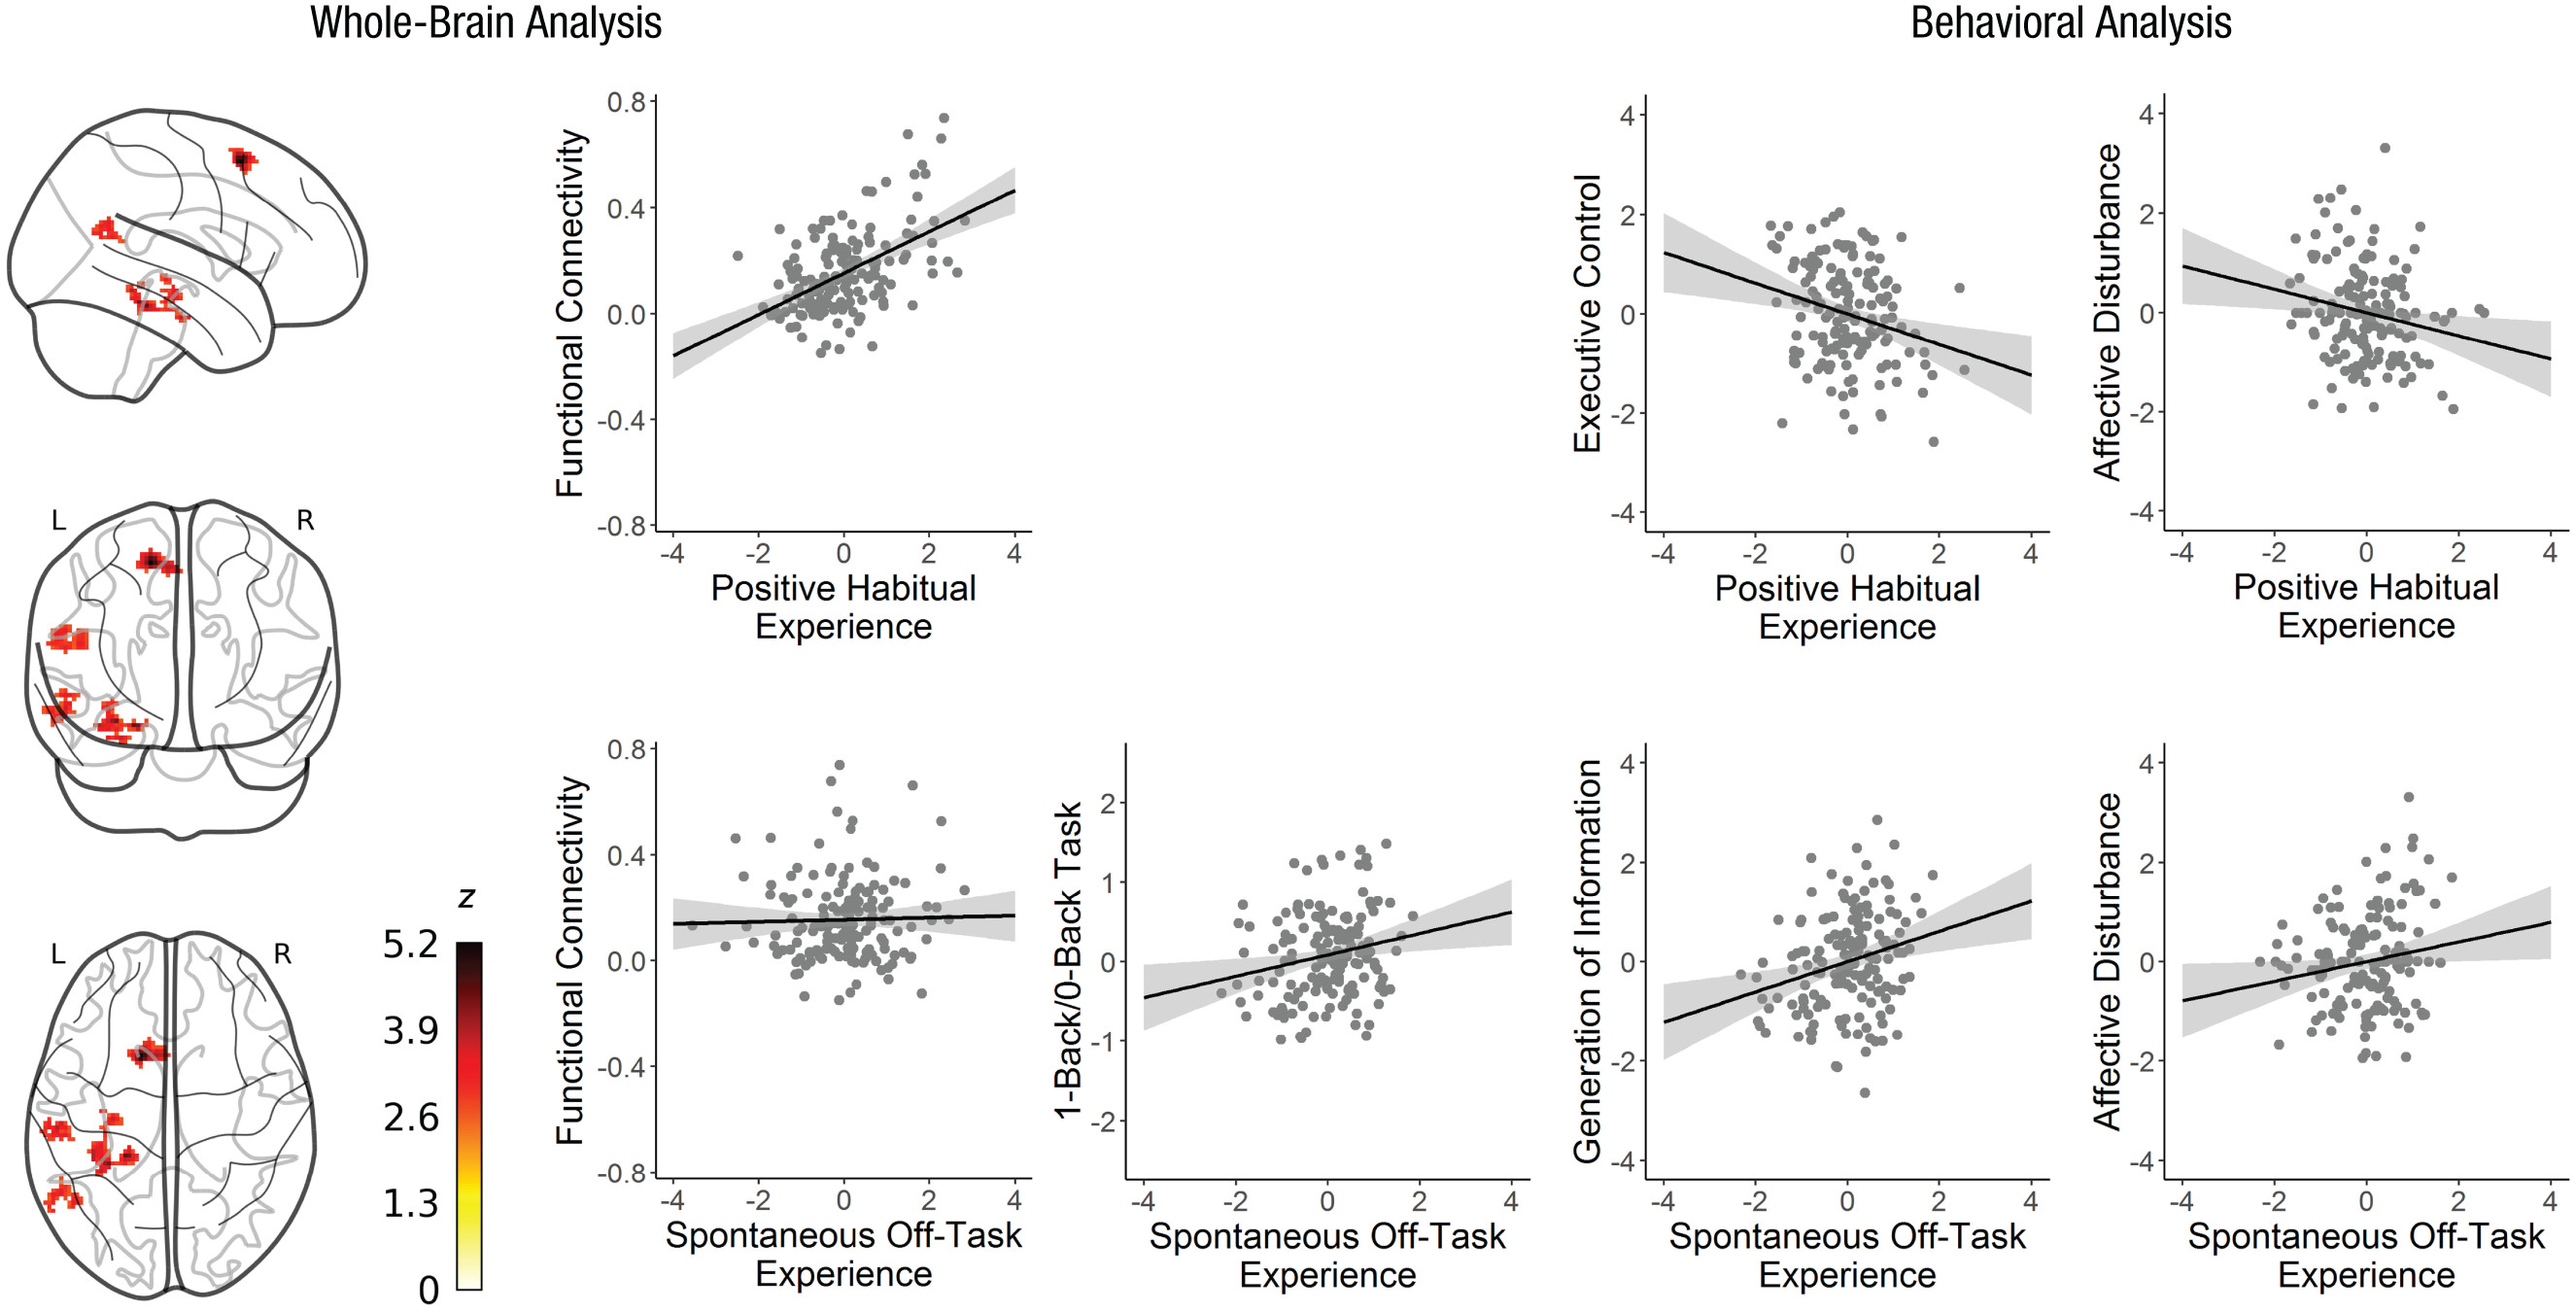
\includegraphics[width=0.8\textwidth]{study1/image/study1fig4.jpeg}
	\caption{Relationship between the different neural-cognitive components and the laboratory and questionnaire measures.}
	\caption*{For the whole-brain analysis, the brain diagrams show clusters of the default-mode-network mask, and the graphs show the correlation between their functional connectivity and the two experience components. For the behavioral analysis, the graphs show the relationship between the two canonical components and measures of well-being and task performance.}

	\label{fig:study1:fig4}
\end{sidewaysfigure}

Next, we explored whether the different canonical components had specific implications for performance on the tasks in which we assessed experience (i.e., the 0-back/1-back task). Because the SCCA depends on resting-state data recorded independently of the task, we were unable to estimate the canonical components separately for each task. Consequently, in these analyses, we explored whether overall differences in canonical component loadings across participants were associated with performance efficiency on the 0-back/ 1-back task. We used a repeated measures analysis of variance in which the dependent variable was the efficiency with which participants performed the 0-back/ 1-back task, respectively. This analysis revealed a significant interaction between task efficiency and variation in our spontaneous-off task component,
\(\mathit{F}(1, 154) = 6.43\),
\(\mathit{p} = .012\),
\(\mparetasquared = .04\).
Decomposition of this interaction showed that participants who scored higher on spontaneous off-task experience performed better on the 0-back condition,
\(\mathit{b} = 0.06\),
\(\text{95\% confidence interval (CI)} = [0.01, 0.11]\),
\(\mathit{t}(151) = 2.38\),
\(\mathit{p} = .019\),
\(\mparetasquared = .04\),
and worse on the 1-back condition,
\(\mathit{b} = -0.09\),
\(\text{95\% CI} = [-0.15, -0.02]\),
\(\mathit{t}(151) = -2.55\),
\(\mathit{p} = .012\),
\(\mparetasquared = .04.\)
The differential relationship between the levels of spontaneous off-task experience and performance on the 0-back/1-back task is shown in Figure \ref{fig:study1:fig4}. These data confirm accounts that suggest that attentional lapses linked to mind wandering are context dependent, tending to have more negative effects as tasks become more demanding \cite{SmallwoodCC2013}; they are also consistent with prior studies suggesting that context regulation may be more problematic for spontaneous than deliberate mind wandering \cite<see also>{SeliTiCS2016}.

Finally, we used MANOVA to determine how the patterns of experience revealed by SCCA were related to the decompositions of the battery of cognitive performance and questionnaire measures. In this analysis, PCA scores describing either phenotypical variation or questionnaire measures on each of the components of cognitive function were the independent variables, and the individual loadings for each of the two canonical components describing experience from the SCCA were the dependent variables. For the analysis of phenotypical variation, this produced two significant results with the executive-control component,
\(\mathit{F}(2, 152) = 5.84\),
\(\mathit{p} = .006\),
\(\mparetasquared = .065\),
and the generation-of-information component,
\(\mathit{F}(2, 152) = 3.41\),
\(\mathit{p} = .007\),
\(\mparetasquared = .065\).
Higher loadings on the positive-habitual component,
\(\mathit{F}(1, 153) = 9.84\),
\(\mathit{p} = .002\),
\(\mparetasquared = .060\),
were associated with worse performance on tasks requiring executive control,
\(\mathit{b} = −0.19\),
\(\text{95\% CI} = [−0.32, −0.07]\),
\(\mathit{t}(153) = −3.14\),
\(\mathit{p} = .002\),
\(\mparetasquared = .060\),
and higher loadings on the spontaneous-off task experience component,
\(\mathit{F}(1, 153) = 10.15\),
\(\mathit{p} = .002\),
\(\mparetasquared = .062\),
were associated with better performance on tasks involving the generation of information (such as creativity),
\(\mathit{b} = 0.20\),
\(\text{95\% CI} = [0.08, 0.33]\),
\(\mathit{t}(153) = 3.19\),
\(\mathit{p} = .002\),
\(\mparetasquared = .062\).
This indicates that two of the experiential components identified by the SCCA were uniquely associated with poor performance on executively demanding tasks and better performance on measures of creativity: both aspects of psychological functioning that have previously been linked to mind wandering \cite<e.g.,>{Baird2012,McVay2009}. The relationships for both neurocognitive dimensions are shown in Figure \ref{fig:study1:fig4}.

In terms of the relationship to the questionnaire decomposition, we found a significant association with the first principal component,
\(\mathit{F}(1, 151) = 3.76\),
\(\mathit{p} = .026\),
\(\mparetasquared = .05\),
which captured affective disturbance. This revealed two significant relationships: (a) a strong association with the positive-habitual component,
\(\mathit{F}(1, 152) = 6.13\),
\(\mathit{p} = .014\),
\(\mparetasquared = .04\),
which suggests a negative association between positive-habitual thought and levels of affective disturbance,
\(\mathit{b} = −0.16\),
\(\text{95\% CI} = [-0.29, 0.03]\),
\(\mathit{t}(152) = −2.48\),
\(\mathit{p} = .04\),
\(\mparetasquared = .062\),
and (b) an association with the spontaneous-off-task-experience component,
\(\mathit{F}(1, 152) = 4.55\),
\(\mathit{p} = .035\),
\(\mparetasquared = .03\),
which suggests that higher loadings on this component were associated with higher levels of affective disturbance,
\(\mathit{b} = 0.15\),
\(\text{95\% CI} = [0.11, 0.28]\),
\(\mathit{t}(152) = 2.13\),
\(\mathit{p} = .035\),
\(\mparetasquared = .03\).
This analysis demonstrates that the different canonical components have dissociable associations with respect to well-being, capturing aspects of the bidirectional relationship between the mind-wandering state and affective disturbance highlighted by prior research \cite<e.g.,>{Killingsworth2010,RubyPlos2013}. Importantly, our analysis demonstrates that the different canonical components have dissociable associations with respect to well-being, which shows that our method captured both elements of the apparently contradictory analysis linking the mind-wandering state to well-being that has been highlighted by prior research.

One concern with resting-state functional connectivity arises from the possibility that the connectivity matrices are unduly affected by individual differences in motion \cite{Power2014}. Consistent with this possibility, our results showed a correlation at the group level between the positive-habitual component,
\(\mathit{r}(155) = .363\),
\(\mathit{p} < .001\),
but not the spontaneous-off-task-experience component,
\(\mathit{r}(155) = −.097\),
\(\mathit{p} = .229\).
Hence, we assessed the contribution of this association to our results linking positive-habitual thought to our measured phenotypes. We performed a series of stepwise analyses to identify the contribution that motion made to the phenotypical associations with positive-habitual thought. In these analyses, the canonical component was the dependent variable. We entered the principal components describing cognition or well-being in the first step and Jenkinson’s mean FD in the second step. Including motion significantly improved the predictive value of the model for well-being--
Model 1:
\(\mathit{R}^{2} = .06\),
\(\mathit{F}(4, 152) = 2.21\),
\(\mathit{p} = .07\),
\(\mparetasquared = .06\);
Model 2:
\(\mathit{R}^{2} = .19\),
\(\mathit{F}(5, 151) = 6.95\),
\(\mathit{p} < .001\),
\(\mparetasquared = .19\);
model change:
\(\mathit{R}^{2} = .13\),
\(\mathit{F}(1, 151) = 24.51\),
\(\mathit{p} < .001\)
--as well as of the model for cognition:
Model 1:
\(\mathit{R}^{2} = .07\),
\(\mathit{F}(3, 153) = 3.92\),
\(\mathit{p} = .010\),
\(\mparetasquared = .07\);
Model 2:
\(\mathit{R}^{2} = .18\),
\(\mathit{F}(4, 152) = 8.22\),
\(\mathit{p} < .001\),
\(\mparetasquared = .18\);
model change:
\(\mathit{R}^{2} = .11\),
\(\mathit{F}(1, 152) = 19.65\),
\(\mathit{p} < .001\).
In the case of well-being, the explained variance of the affective disturbance component was not improved with the inclusion of motion--
Model 1: affective-disturbance
\(\beta = -0.20\),
\(\mathit{t}(152) = −2.48\),
\(\mathit{p} = .014\),
\(\mparetasquared = .04\),
\(\text{95\% CI} = [−0.29, −0.03]\);
Model 2: affective-disturbance
\(\beta = −0.20\),
\(\mathit{t}(151) = −2.59\),
\(\mathit{p} = .011\),
\(\mparetasquared = .05\),
\(\text{95\% CI} = [−0.28, −0.03]\),
Model 2: mean-FD
\(\beta = 0.36\),
\(\mathit{t}(151) = 4.94\),
\(\mathit{p} < .001\),
\(\mparetasquared = .14\),
\(\text{95\% CI} = [3.29, 7.67]\).
Thus, the relationship between affective disturbance and positive-habitual thought remained largely unchanged by the inclusion of motion as a nuisance variable. In the case of cognition, executive control accounted for less variance in the positive-habitual component when mean FD was included--
Model 1: executive-control
\(\beta = −0.24\),
\(\mathit{t}(153) = −3.14\),
\(\mathit{p} = .002\),
\(\mparetasquared = .06\),
\(\text{95\% CI} = [−0.32, −0.07]\);
Model 2: executive-control
\(\beta = −0.16\),
\(\mathit{t}(152) = −2.17\),
\(\mathit{p} = .032\),
\(\mparetasquared = .03\),
\(\text{95\% CI} = [−0.25, −0.01]\);
Model 2:
\(\beta = −0.34\),
\(\mathit{t}(152) = 4.43\),
\(\mathit{p} < .001\),
\(\mparetasquared = .11\),
\(\text{95\% CI} = [4.82, 12.56]\).

Unlike in the well-being analysis, motion explained a substantial amount of variance that was shared in the relationship between executive control and positive-habitual thought. To explore whether the positive-habitual component reflected an artefact of motion, we selected participants for whom movement greater than 0.2 mm occurred on less than 5\% of the resting-state data (\(\mathit{N}\) = 134) and reran the SCCA with the identical pipeline. This produced similar solutions for both positive-habitual and spontaneous off-task thought (see Fig.\ref{fig:3S4} in the Supplemental Material \ref{appendix:study1:subsection3}). Importantly, positive-habitual thought was not significantly correlated with motion,
\(\mathit{r}(132) = .10\),
\(\mathit{p} = .236\),
but was correlated with poor executive control,
\(\mathit{r}(155) = -.26\),
\(\mathit{p} = .001\)
(see Table \ref{tab:S1} in the Supplemental Material \ref{appendix:study1:subsection3} for the full set of correlations).
This final analysis shows that in a more restricted sample in which motion did not correlate with either latent component, we still observed a relationship between positive-habitual thought and poor executive control.

% ==========================================================================================================
\section{Discussion}
\label{study1:discussion}
Using multivariate pattern analysis, our study demonstrated that the content of the mind-wandering state is heterogeneous and confirmed hypotheses that different types of experience have differing functional associations \cite{SmallwoodCC2013}.
Using a novel analysis strategy, we simultaneously decomposed self-reports of experience with descriptions of neural organisation, revealing dimensions of experience with unique phenotypical associations: positive-habitual experiences and spontaneous off-task thoughts.

Poor executive control, a well-documented association of mind wandering \cite{McVay2009},
predicted variation in positive-habitual thoughts. This pattern of thinking was linked to coupling in the mPFC, a region important for assigning value to neural signals \cite{Roy2012}.
It is possible that deficits in executive control during mind wandering emerge because of problems in assigning value to an external task, a view supported by evidence that financial motivation limits the impact of mind wandering on performance \cite{MrazekJoEP2012}.
We found that spontaneous off-task experiences simultaneously underlie the association between mind wandering and tasks of creativity \cite{Baird2012},
as well as problems in performing tasks requiring continuous monitoring of external information. Finally, while positive-habitual experiences are linked to improved well-being, spontaneous off-task experiences are associated with increased affective disturbance, which captures the apparent contradiction that mind wandering can be associated with both negative \cite<e.g.,>{Killingsworth2010}
and positive \cite<e.g.,>{PoerioFrontiers2016}
emotional states. Together, these data provide the most convincing evidence to date that experience during mind wandering unfolds along a set of underlying dimensions and that these explain many of the phenotypical associations that have hitherto been associated with the mind-wandering state \cite{SmallwoodCC2013}.

Our study also demonstrates the complex contribution that the DMN makes to cognition. Strong DMN connectivity at rest was associated with an increased tendency for positive-habitual thoughts about the future, which corroborates previous research linking the DMN to mental time travel \cite{Karapanagiotidis2017,Schacter2007}. Participants also rated these experiences as habitual, a pattern that supports accounts of the role of the DMN in cognition as emphasising automatic influences during mind wandering \cite{Christoff2016}. Spontaneous off-task thoughts, in contrast, showed weaker integration between core DMN regions and were linked to poor performance in the 1-back condition, a context in which task performance depends on the DMN functioning as a coherent network \cite{Konishi2015}. More generally, we found that states of high connectivity within the DMN (positive-habitual thoughts) were associated with more functional coupling to regions outside of the core network—a key prediction of the view that activity within the DMN reflects the integration of information from across the cortex \cite{Margulies2016}.
It is important to note that our analysis shows that the behavior of the DMN at rest contains information about individual variation in the type of experiences that emerge during mind wandering. These data should not be taken as evidence that this system is exclusive in its role in mind wandering. Indeed, our whole-brain regression provides quantitative evidence that the interactions of the DMN with other regions, including those in the medial temporal lobe and the executive system (e.g., pre-SMA), are also important. In this way, our study supports recent theoretical perspectives \cite<e.g.,> {Christoff2016,Margulies2016},
as well as prior empirical results \cite<e.g.,>{Ellamil2016,Golchert2017,Smallwood2016}
highlighting that regions other than the DMN core are important for mind wandering.

There are a number of limitations of the current analysis. First, our study focused on describing mind wandering as a trait. Prior work has shown similarities between state and trait measures of mind wandering in terms of (a) neural processing (e.g., trait: \citeNP{Smallwood2016};  state: \citeNP{Christoff2009,StawarczykPlos2011})
and (b) psychological processes such as working capacity
(e.g., trait: \citeNP{McVay2009}; state: \citeNP{MrazekJoEP2012})
and happiness
(e.g., trait: \citeNP{RubyPlos2013}; state: \citeNP{Killingsworth2010}).
Nonetheless there are certain aspects of mind wandering that can be understood only by treating it as a state, such as its temporal features
\cite{Christoff2016}.
Second, our study measured mind wandering in the laboratory. Although there is a correspondence between mind wandering in laboratory and naturalistic settings \cite<e.g.,>{McVay2009},
its form and content may depend on the contexts in which the experience emerges. Consequently, our findings should be supplemented by studies examining the occurrence of different types of experience in ecologically valid settings. Finally, our study did not find evidence for links with tasks that rely on semantic memory or for links to psychological traits other than well-being. This may have been due to our selection of neural regions or from our selection of questions. Prior studies have linked regions in the temporal lobe to the contents of thought \cite<e.g.,>{Smallwood2016},
a pattern of data that is consistent with a role of the semantic system in spontaneous thought \cite{Binder2009}.
Other work has highlighted awareness of mind wandering as important in traits such as hyperactivity \cite{Franklin2017}.
We anticipate that extending the selected regions of the cortex and the aspects of experience measured may extend our understanding of the mind wandering state to encompass forms of semantic processing and additional psychological traits.

In closing, our study provides the strongest evidence to date that the mind-wandering state is heterogeneous in its content, neural basis, and functional associations. We describe two neurocognitive dimensions capturing associations with attentional lapses, creativity and well-being, confirming much of the research on mind wandering conducted over the last decade. However, we also provide an explanation for why scientific accounts of mind wandering have been dominated by controversy, such as its relationship to
happiness \cite{Killingsworth2010},
creativity \cite{Smeekens2016},
executive control \cite{McVay2009},
and the DMN \cite{Gilbert2007}.
Our data suggest that these debates emerge from an erroneous assumption that mind wandering is a unitary psychological construct, when it is in fact made up of distinct states with unique neural correlates and functional associations. This ontological uncertainty has led to artificial controversies that hinder the development of a mature science of internal experience. Although our findings do not capture the full range of experiential dimensions on which the mind can wander, they convincingly demonstrate that it is untenable to characterise mind wandering as a uniform experience. As a discipline, we must embrace methodologies and analytical techniques that capture the complex nature of internal experiences, allowing researchers to accurately determine the contribution that they make to people’s lives.

% ==========================================================================================================
